\documentclass[../main.tex]{subfiles}
\begin{document}
\newpage
\section{Определение и элементарные свойства определенного интеграла: аддитивность, монотонность, оценка модуля, частный случай первой теоремы о среднем.}
Определённый интеграл можно вводить по-разному, но в конечном итоге всё это приводит к одному и тому же набору свойств. 
Мы будем вводить его через площадь подграфика. 

\( \Let \; f \in C\left[ a,b\right],\quad \forall \; x\;\; f\left( x\right) \geq 0\). Площадью подграфика называется отображение, которое сопоставляет 
паре \( (f,\; \left[ a,b\right])\) некоторое неотрицательное число
\[ \left( f,\left[ a,b\right]\right) \longmapsto S\left( f, \left[ a,b\right]\right) \geq 0\]
и удовлетворяет 3 аксиомам:
\begin{enumerate}
    \item \emph{Аддитивность относительно промежутка.} \( \forall \; f \in C\left[ a,b\right],\quad \forall \; c \in \left( a,b\right)\)
    \[ S\left( f, \left[ a,b\right]\right)=S\left( f, \left[ a,c\right]\right)+S\left( f, \left[ c,b\right]\right)\]
    \item \emph{Монотонность.} \( \forall \; f,g \in C\left[ a,b\right],\quad \forall \; x \in \left[ a,b\right]\)
    \[ f\left( x\right) \leq g\left( x\right) \implies S\left( f,\left[ a,b\right]\right) \leq S\left( g,\left[ a,b\right]\right)\] 
    \item \emph{Нормированность.} \( \forall \; x \in \left[ a,b\right]\)
    \[ f\left( x\right)=k \implies S\left( f,\left[ a,b\right]\right)=k \cdot \left( b-a\right)\] 
\end{enumerate}

Стоит ещё раз подчеркнуть, что площадь подграфика определяется только для неотрицательных функций. 

\begin{note}
    \hypertarget{note:pm}{~}
    Пусть \( x \in \R \). Обозначим \( x_+= \max\limits_{ } \left( x, 0\right),\quad x_-= \max\limits_{ } \left( -x, 0\right)\). Тогда
    \[ x_+ - x_-=x,\quad x_+ +x_-=\left| x\right|,\quad x_+,x_- \geq 0,\quad x_+, x_- \leq \left| x\right|\]
\end{note}

Применим это замечание к функциям: если \( f\) - функция, то пусть 
\[ f_+\left( x\right)= \max\limits_{ } \left( f\left( x\right),0\right),\quad f_-\left( x\right)= \max\limits_{ } \left( -f\left( x\right),0\right)\]

\begin{note}
    \[ f \in C\left[ a,b\right] \implies f_+,f_- \in C\left[ a,b\right]\]
\end{note}

\begin{center}
    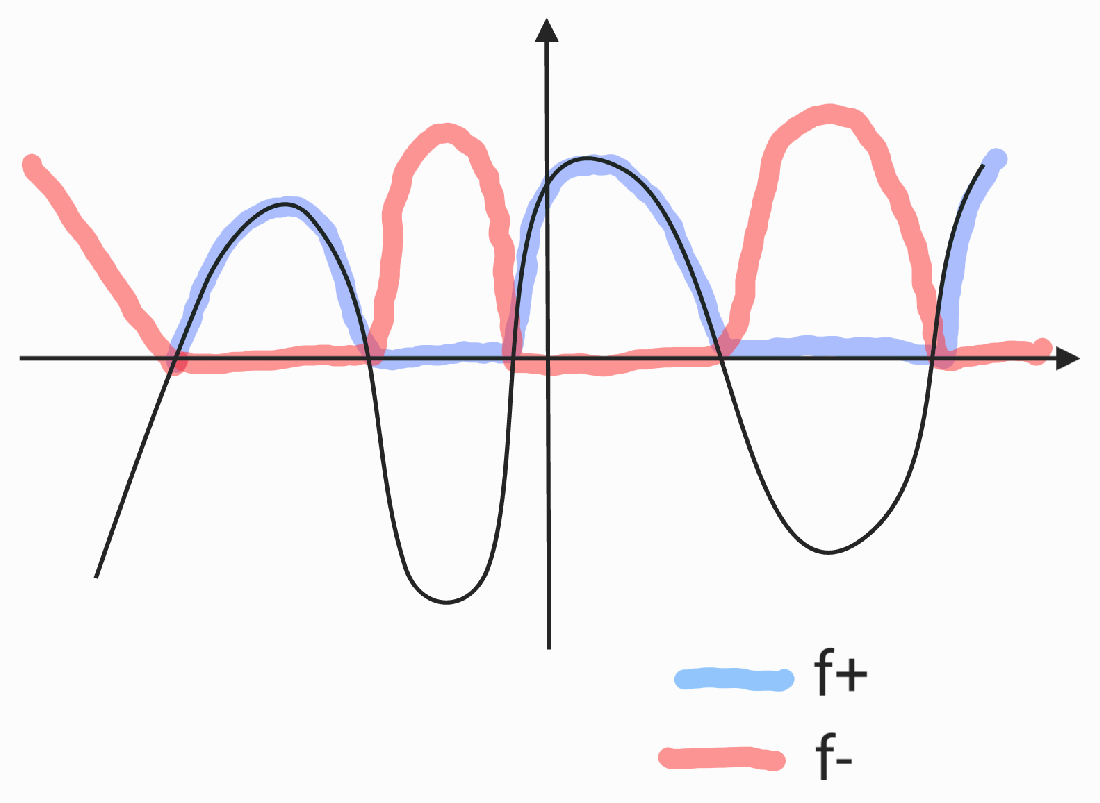
\includegraphics[width=0.6\linewidth]{15_functions.pdf}
\end{center}

\emph{Определённый интеграл} определяется следующий образом: 
\[ \displaystyle\int\limits_{ a}^{ b} f\left( x\right)dx = S\left( f_+, \left[ a,b\right]\right)-S\left( f_-, \left[ a,b\right]\right)\] 

\begin{prop}{\hypertarget{thm:def_int_prop}{Свойства определённого интеграла}}
    \begin{enumerate}
        \item Аддитивность относительно промежутка. \( \forall \; \left[ a,b\right],\quad \forall \; f \in C\left[ a,b\right],\quad \forall \; c \in \left( a,b\right)\)
        \[ \displaystyle\int\limits_{ a}^{ b} f\left( x\right)dx= \displaystyle\int\limits_{ a}^{ c} f\left( x\right)dx + \displaystyle\int\limits_{ c}^{ b} f\left( x\right)dx\]
        \item Монотонность. \( \forall \; f,g \in C\left[ a,b\right]: \quad \forall \; x \in \left[ a,b\right]\quad f\left( x\right) \leq g\left( x\right)\)
        \[ \displaystyle\int\limits_{ a}^{ b} f\left( x\right)dx \leq \displaystyle\int\limits_{ a}^{ b} g \left( x\right)dx\]
        \item Нормированность. \( \forall \; x \in \left[ a,b\right]\)
        \[ f\left( x\right)=k \implies \displaystyle\int\limits_{a }^{ b} f\left( x\right)dx=k \cdot \left( b-a\right)\]
        \item Оценки интеграла. \( \Let \; f \in C\left[ a,b\right]\)
        \[ \forall \; x \in \left[ a,b\right]\quad  m \leq f\left( x\right) \leq M \implies m \cdot \left( b-a\right) \leq \displaystyle\int\limits_{ a}^{ b} f\left( x\right)dx \leq M \cdot \left( b - a\right)\]
        \item Если \( f \in C\left[ a,b\right],\quad \forall \; x \in \left[ a,b\right]\quad f\left( x\right) \geq 0\) и \( \exists \; x_0 \in \left[ a,b\right]:\quad f\left( x\right)>0\), тогда
        \[ \displaystyle\int\limits_{ a}^{ b} f\left( x\right)dx >0\]
    \end{enumerate}
\end{prop}

\begin{proof}
    
    ~

    \begin{enumerate}
        \item \begin{equation*}
            \begin{aligned}
                &\displaystyle\int\limits_{ a}^{ b} f\left( x\right)dx=S\left( f_+, \left[ a,b\right]\right)-S\left( f_-, \left[ a,b\right]\right)=\left( S\left( f_+, \left[ a,c\right]\right)+S\left( f_+, \left[ c,b\right]\right)\right)-\\
                &-\left( S\left( f_-,\left[ a,c\right]\right)+S\left( f_-, \left[ c,b\right]\right)\right)=\\ 
                &=\left( S\left( f_+, \left[ a,c\right]\right)-S\left( f_-,\left[ a,c\right]\right)\right)+\left( S\left( f_+, \left[ c,b\right]\right)-S\left( f_-, \left[ c,b\right]\right)\right)= \\
                &=\displaystyle\int\limits_{ a}^{ c} f\left( x\right)dx+ \displaystyle\int\limits_{ c}^{ b} f\left( x\right)dx
            \end{aligned}
        \end{equation*}
        \item Сначала отметим такой факт: \( h\left( x\right) \geq 0 \implies \displaystyle\int\limits_{ a}^{ b} h\left( x\right)dx=S\left( h_+, \left[ a,b\right]\right)\), потому что \( h_-\) это тождественный 0 и площадь её подграфика равна 0. 
        \begin{equation*}
            \begin{aligned}
                &f\left( x\right) \leq g \left( x\right) \implies \max\limits_{ } \left( f\left( x\right),0\right) \leq \max\limits_{ } \left( g \left( x\right),0\right) \implies f_+\left( x\right) \leq g_+ \left( x\right) \implies \\
                & \implies S\left( f_+, \left[ a,b\right]\right) \leq S\left( g_+, \left[ a,b\right]\right)\\ \\
                & f\left( x\right) \leq g \left( x\right) \implies \max\limits_{ } \left( -f\left( x\right),0\right) \geq \max\limits_{ } \left( -g \left( x\right),0\right) \implies f_-\left( x\right) \geq g_- \left( x\right) \implies \\
                & \implies S\left( f_-, \left[ a,b\right]\right) \geq S\left( g_-, \left[ a,b\right]\right)
            \end{aligned}
        \end{equation*}
        \begin{equation*}
            \begin{cases}
                S\left( f_+, \left[ a,b\right]\right) \leq S\left( g_+, \left[ a,b\right]\right)\\
                S\left( f_-, \left[ a,b\right]\right) \geq S\left( g_-, \left[ a,b\right]\right)
            \end{cases}
            \implies
            S\left( f_+,\left[ a,b\right]\right)-S\left( f_-,\left[ a,b\right]\right) \leq S\left( g_+, \left[ a,b\right]\right)-S\left( g_-,\left[ a,b\right]\right)
        \end{equation*}
        \[S\left( f_+,\left[ a,b\right]\right)-S\left( f_-,\left[ a,b\right]\right) \leq S\left( g_+, \left[ a,b\right]\right)-S\left( g_-,\left[ a,b\right]\right) \implies \displaystyle\int\limits_{ a}^{ b} f\left( x\right)dx \leq \displaystyle\int\limits_{ a}^{ b} g \left( x\right)dx\]
        \item Пусть \( f\left( x\right)=k\) на \( \left[ a,b\right]\). \\
        Если \( k \geq 0 \implies f_-\equiv 0 \implies S\left( f_-,\left[ a,b\right]\right)=0 \implies \displaystyle\int\limits_{ a}^{ b} f\left( x\right)dx=S\left( f_+,\left[ a,b\right]\right)=k \cdot \left( b-a\right)\)\\
        Если \( k < 0 \implies f_+\equiv 0 \implies S\left( f_+,\left[ a,b\right]\right)=0 \implies \displaystyle\int\limits_{ a}^{ b} f\left( x\right)dx=-S\left( f_-,\left[ a,b\right]\right)=k \cdot \left( b-a\right)\)
        \item Рассмотрим функции \( g_m\left( x\right)=m,\quad g_M\left( x\right)=M\quad \forall \; x \in [a,b]\).
        \[ g_m\left( x\right) \leq f\left( x\right) \leq g_M\left( x\right)\]
        \par Пользуясь 2 и 3 свойствами интеграла, получаем:
        \[ m \cdot \left( b-a\right) = \displaystyle\int\limits_{ a}^{ b} g_m\left( x\right)dx \leq \displaystyle\int\limits_{ a}^{ b} f\left( x\right)dx \leq \displaystyle\int\limits_{ a}^{ b} g_M\left( x\right)dx=M \cdot \left( b-a\right)\]
        \item Если \( x_0\) - это крайняя точка отрезка \( \left[ a,b\right]\), то по теореме о стабилизации знака существует окрестность точки \( x_0\), в которой \(f\left( x\right) >0\). Тогда возьмём и переприсвоим точке \( x_0\) значение любой другой точки из этой окрестности, чтобы она не была крайней точкой отрезка. 
        \par Теперь можем считать, что \( x_0 \in \left( a,b\right)\). Опять же по теореме о стабилизации знака 
        \[ f\left( x_0\right)=A>0,\quad \exists \; \delta \in \left( 0, b-x_0\right): \;\forall \; x \in \underbrace{\left( x_0, x_0+ \delta \right)}_{ \subseteq  \left( x_0, b\right)}\quad f\left( x\right)> \dfrac{ A}{ 2} \]
        \par Тогда получаем:
        \[ \displaystyle\int\limits_{ a}^{ b} f\left( x\right)dx= \underbrace{\displaystyle\int\limits_{ a}^{ x_0} f\left( x\right)dx}_{ \geq 0}+ \underbrace{\displaystyle\int\limits_{ x_0}^{ x_0+ \delta }f\left( x\right)dx }_{ \geq \frac{ A}{ 2} \cdot \delta  }+ \underbrace{\displaystyle\int\limits_{ x_0+ \delta}^{ b}f \left( x\right)dx}_{ \geq 0} \geq \dfrac{ A}{ 2} \cdot \delta >0 \]
    \end{enumerate}
\end{proof}

В интеграле \( \displaystyle\int\limits_{ a}^{ b} f\left( x\right)dx\) есть неявное ограничение, что \( \left[ a,b\right]\) - отрезок, то есть \( a \leq b\). Мы хотим убрать это ограничение. 
Для этого при \( a > b\) полагают \( \displaystyle\int\limits_{ a}^{ b} f\left( x\right)dx = - \displaystyle\int\limits_{ b}^{ a} f\left( x\right)dx\). Все свойства интеграла при этом сохраняются (доказательство - разбор случаев).

\begin{thm}[\hypertarget{thm:simple_average}{Теорема о среднем}]
    \( \Let \; f \in C\left[ a,b\right]\)

    Тогда 
    \[ \exists \; c \in \left[ a,b\right]:\quad \displaystyle\int\limits_{ a}^{ b} f\left( x\right)dx = f\left( c\right) \cdot \left( b-a\right)\]
\end{thm}

\begin{proof}
    
    ~

    Из 4 свойства определённого интеграла мы знаем, что \( \dfrac{ \displaystyle\int_{a}^{b}f\left(x\right)fx}{ b-a} \in \left[ \min\limits_{ \left[ a,b\right]}f, \max\limits_{ \left[ a,b\right]} f \right]\). По теореме Вейерштрасса функция \( f\), непрерывная 
    на отрезке, достигает на нём своего минимума и максимума. А по теореме Коши-Больцано о промежуточном значении, она должна принимать и все значения между минимумом и максимумом. Значит
    \[ \exists \; c \in \left[ a,b\right]:\quad \dfrac{ \displaystyle\int_{a}^{b}f\left(x\right)dx}{ b-a} = f(c)\]
    \[ \displaystyle\int\limits_{ a}^{ b} f\left( x\right)dx = f(c) \cdot \left( b-a\right)\]
\end{proof}

\begin{thm}[Оценка модуля интеграла]
    \( \Let \; f \in C\left[ a,b\right]\).

    Тогда
    \[ \left| \displaystyle\int\limits_{ a}^{ b} f\left( x\right)dx\right| \leq \displaystyle\int\limits_{ a}^{ b} \left| f\left( x\right)\right|dx\]
\end{thm}

\begin{proof}
    
    ~

    Из свойств модуля \( -\left| f\left( x\right)\right| \leq f\left( x\right) \leq \left| f\left( x\right)\right|\). По монотонности интеграла мы знаем, что тогда 
    \[ \displaystyle\int\limits_{ a}^{ b} \left( -\left| f\left( x\right)\right|\right)dx \leq \displaystyle\int\limits_{ a}^{ b} f\left( x\right)dx \leq \displaystyle\int\limits_{ a}^{ b} \left| f\left( x\right)\right|dx\]

    Дальше нужно вынести минус в левой части неравенства, но про линейность определённого интеграла мы пока не знаем и не можем на неё сослаться. Поэтому нужно доказать отдельно, что минус можно вынести. Пусть некоторая функция \( g \in C\left[ a,b\right],\quad g \left( x\right) \geq 0\quad \forall \; x \in \left[ a,b\right]\). Тогда
    \[\displaystyle\int\limits_{ a}^{ b} -g \left( x\right)dx=S\left( (-g)_+, \left[ a,b\right]\right) - S\left( (-g)_-, \left[ a,b\right]\right)=S\left( g_-, \left[ a,b\right]\right)-S\left( g_+, \left[ a,b\right]\right)=- \displaystyle\int\limits_{ a}^{ b} g \left( x\right)dx\]

    Теперь можем вынести минус, получим:
    \[ - \displaystyle\int\limits_{ a}^{ b} \left| f\left( x\right)\right|dx \leq \displaystyle\int\limits_{ a}^{ b} f\left( x\right)dx \leq \displaystyle\int\limits_{ a}^{ b} \left| f\left( x\right)\right|dx\]

    И по свойству модуля это равносильно
    \[ \left| \displaystyle\int\limits_{ a}^{ b} f\left( x\right)dx\right| \leq \displaystyle\int\limits_{ a}^{ b} \left| f\left( x\right)\right|dx\]
\end{proof}
\end{document}